\chapter{Multiparty Cardinality Testing}

Der Fokus dieser Arbeit liegt auf dem MPCT Protokoll, das von Branco et al. im Jahr 2021 \cite{Doettling2021} vorgestellt wurde. Es gab schon vorher einige Veröffentlichungen zum Thema Private Set Intersections, auf denen das Paper aufbauen konnte. Zuerst wurden Protokolle für zwei Parteien entworfen, dann auch für mehrere Parteien. Das Paper von Gosh und Simkin \cite{Ghosh2019} ist die neuste Veröffentlichung, auf der das Protokoll aufbaut.\\
Die große Neuerung von Gosh und Simkin ist, dass die Kommunikations-Komplexität nun vor allem von O(t) (also dem threshold, oder der Anzahl an "erlaubten Abweichungen") und nur noch logarithmisch von O(n) (also der Größe der Eingabemengen) abhängt. \cite{Ghosh2019}\\
Das von Gosh vorgeschlagene Cardinality Testing ist jedoch noch nicht  für mehrere Parteien optimiert. Daher ist das neue Protokoll zur Bestimmung der Schnittmengen-größe die wichtigste Neuerung des Papers \cite{Doettling2021}.

\section{Wie das MPCT Protokoll funktioniert}
Jede Partei wandelt ihre Eingabemenge in ein Polynom um. Dieses Polynom wird dann an 4t+2 Stellen ausgewertet. Die verschlüsselten Punkte können dann an die anderen Teilnehmer geschickt werden. Eine der Parteien teilt dann die Summe der erhaltenen Ergebnisse für einen Punkt durch den wert des Eigenen Polynoms an diesem Punkt.
Die Ergebnisse dieser Berechnung werden dann an das Teil-Protokoll SDT geschickt, das berechnen soll, ob der Grad des Zählers und des Nenners kleiner oder gleich t ist.\\
SDT erstellt aus den erhaltenen verschlüsselten Zahlen dann ein lineares System. Mithilfe der Teil-Protokolle secRank und OLS werden erst Eigenschaften des linearen Systems getestet und dann wird das System gelöst. Aus der Lösung des Systems werden zuletzt noch Polynome gebildet und miteinander verrechnet. Wenn diese an einem Punkt ausgewertet 0 ergeben, dann war der Grad von Zähler und Nenner gleich und kleiner oder gleich t.\\
Und wenn das der Fall ist, dann war die Schnittmenge der Eingabemengen größer als t.


\section{Abwandlungen des Protokolls} \label{Änderungen}
\subsection{Broadcasts}
Das Protokoll wurde offensichtlich entworfen, um auch mit mehreren teilnehmenden Parteien effizient zu sein.
Das Paper \cite{Doettling2021} nutzt also in vielen Unterprotokollen Broadcast-Funktionen.

\begin{lstlisting}[firstnumber=1, caption = 
Beispiel: Ausschnitt von secRank \cite{Doettling2021}]
Each party Pi broadcasts an encrypted uniformly chosen at
random unit upper and lower triangular Toeplitz matrices...
\end{lstlisting}

Ich habe versucht, nah an die Spezifizierungen des Papers zu kommen, doch 
um die Implementierung des Protokolls zu vereinfachen und um das Testen der Implementierung zu erleichtern, habe ich das System ein wenig abgewandelt. In meiner Implementierung gibt es einen Koordinator. Dieser Koordinator erleichtert das Testen enorm, denn durch ihn kann sicher gestellt werden, dass alle "verschickten" Informationen immer zum richtigen Zeitpunkt am richtigen Ziel ankommen.\\
Diese Änderung wird die Sicherheit des Protokolls nicht schwächen, weil alle Informationen, die per Broadcast verschickt werden, immer verschlüsselt sind.
Auch wenn Daten entschlüsselt werden, sind sie immer für einen Angreifer, der Informationen über die Eingabemengen erhalten will, nutzlos. Ein gutes Beispiel dafür ist das Unterprotokoll secInv \\

\begin{figure}[h]
\begin{center}
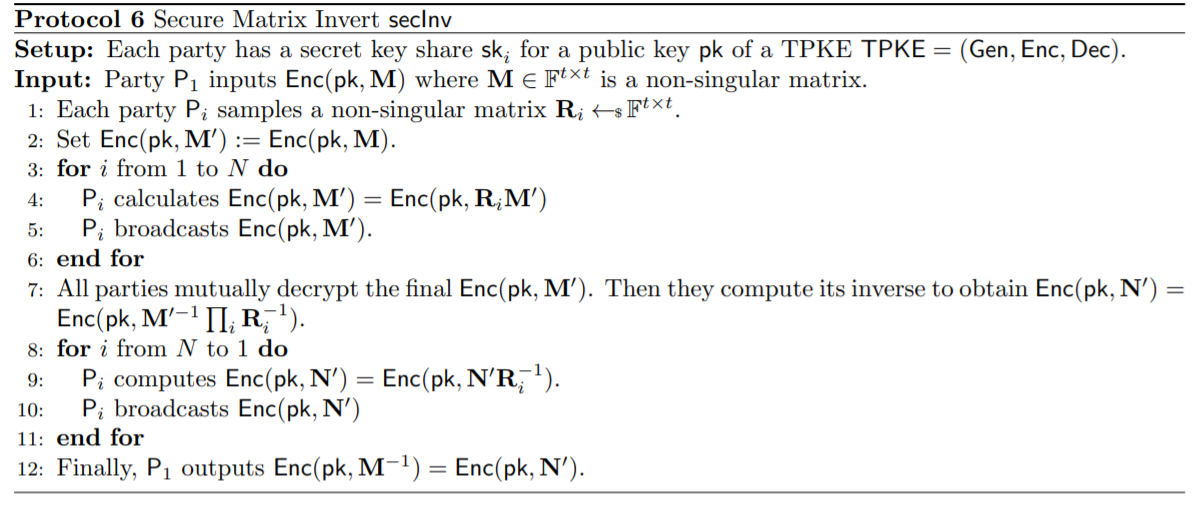
\includegraphics[width = 15cm]{secInv.png}
\caption{Teil-Protokoll secInv}
\cite{Doettling2021}
\label{oInv}
\end{center}

\end{figure}

Hier wird zwar eine Matrix entschlüsselt (7), diese ist aber randomisiert(1-5), also nutzlos, außer, man besitzt eine der geheimen Matrizen(9), die ja nicht verschickt werden.\\
Das Protokoll ist also auf eine Art und Weise aufgebaut, dass kein passiver Zuhörer irgendwelche nützlichen Informationen aus den Nachrichten, die zwischen den Parteien verschickt werden, gewinnen kann. Also kann auch ein Angreifer, der alle Nachrichten zwischen den Teilnehmern des Protokolls erhält, keine Informationen extrahieren. Daher können wir auch sicher sein, dass, selbst wenn der Koordinator von einem Angreifer kontrolliert wird, die verschlüsselten Eingabedaten sicher sind.\\
Die neue Struktur, die einfacher zu implementieren und testen ist, macht das Protokoll also nicht weniger sicher. Besonders deshalb, weil das Protokoll so konstruiert ist, dass selbst alle verschickten Nachrichten zusammen keine geheimen Daten preisgeben.\\
Diese Änderung wird die Analyse der Protokolle nicht beeinflussen, da der Fokus meiner Analyse auf der Anzahl und der Art der Berechnungen liegt und nicht auf der Kommunikationskomplexität. Die Kommunikationskomplexität der Protokolle wurde schon von Branco et al. berechnet und wird deshalb in dieser Arbeit nicht betrachtet. Die Berechnungen sollten von dieser Änderung nicht beeinflusst werden, weshalb die Ergebnisse nicht verfälscht werden sollten.

\subsection{Koordinieren der Parteien}
Die meisten der Unterprotokolle bestehen aus sich abwechselnden Teilen von Kommunikation zwischen den Parteien und Berechnungen der Parteien. Also habe ich die Unterprotokolle implementiert, indem die Berechnungen der Parteien in Abschnitte aufgeteilt sind, die dann von dem Koordinator aufgerufen werden können. Gut zu sehen ist das beispielsweise im Teil-Protokoll MPCT, wo der Koordinator nur die Koordinierung der Parteien übernimmt, indem die Parteien die richtigen Eingaben zum richtigen Zeitpunkt bekommen.\\

\begin{lstlisting}[caption = Ausschnitt der Implementierung von MPCT (vereinfacht)]
public boolean MPCT(List<BigInteger> inputAlphas, BigInteger setMod){

        List<List<EncryptedNumber>> encPointsList = new LinkedList<>();
        //line 1 already done in setup

        //line 2
        for (int i = 0; i < parties.size(); i++) {
            encPointsList.add(parties.get(i).MPCTpart1(inputAlphas, setMod));
        }
        //line 3
        return parties.get(0).MPCTpart2(encPointsList, inputAlphas, t);
    }

\end{lstlisting}

Das ist die einfachste Möglichkeit, um zu erreichen, dass alle Parteien zum richtigen Zeitpunkt das Richtige berechnen, denn einige der Berechnungen hängen auch von den gesendeten Nachrichten der anderen Parteien ab.\\

\section{Ähnliche Veröffentlichungen}
Es gibt einige andere Veröffentlichungen in den letzten Jahren, die sich mit ähnlichen Problemen oder sogar dem gleichen Problem beschäftigen.
Das Problem der Private Threshold Set Intersection lässt sich in zwei Teilprobleme aufteilen. Zum Einen in das Berechnen der Schnittmenge, worauf Gosh sich in \cite{Ghosh2019} konzentriert, und das sogar noch erweitert wurde, um auch für mehr als 2 Parteien nutzbar zu sein \cite{Doettling2021}. Und zum Anderen in der Ermittlung der Größe der Schnittmenge. Das ist der Fokus von Branco et al.  \cite{Doettling2021}. Aber auch Badrinarayanan et al. \cite{cryptoeprint:2020:600} beschäftigen sich mit der Ermittlung der Größe der Schnittmenge. Badrinarayanan nutzt jedoch andere kryptographische Annahmen und erhält die Ergebnisse mithilfe von anderen mathematischen Grundlagen \cite{Doettling2021}.\\
Es gibt also viele neue Entwicklungen in diesem Bereich, die für unterschiedliche Zwecke genutzt oder kombiniert werden können, um die besten Ergebnisse zu erreichen. Das Protokoll aus \cite{Doettling2021} ist also eine relevante Neuerung, und eine Analyse kann helfen, die Effizienz dieser Neuerung mit anderen zu vergleichen.
